\documentclass[11pt]{article}
\usepackage[T1]{fontenc}
\usepackage[german]{babel}
\usepackage[utf8]{inputenc}

%% margins
\usepackage{geometry}
\geometry{
  left=2.5cm,
  right=2.5cm,
  top=2.5cm,
  bottom=2.5cm
}

%% ams/thm
\usepackage{amsmath, amssymb, amsthm, mathtools, cancel, graphicx, wrapfig}

%%\begin{thm config/technicalities}
\theoremstyle{plain}
\newtheorem{thm}{Satz}[section]
\newtheorem{lem}[thm]{Lemma}
\newtheorem*{prop}{Proposition}
\newtheorem*{cor}{Korollar}
\newtheorem*{beh}{Behauptung}

\theoremstyle{definition}
\newtheorem{defn}[thm]{Definition}
\newtheorem{exmp}[thm]{Beispiel}

\theoremstyle{remark}
\newtheorem*{rem}{Bemerkung}

\usepackage{thmtools}

\declaretheoremstyle[%
  spaceabove=1.5ex,%
  spacebelow=6pt,%
  headfont=\normalfont\itshape,%
  postheadspace=1em,%
  qed=\qedsymbol%
]{mystyle} 
\declaretheorem[name={Beweis},style=mystyle,unnumbered,
]{prf}

\renewcommand{\proof}{\prf}

%% paragraph spacing/indentation
\usepackage{parskip}
\usepackage{setspace}
\setlength{\parindent}{0cm}

\makeatletter
\def\thm@space@setup{%
  \thm@preskip=\parskip \thm@postskip=0pt
}
\makeatother
%\end{}

%% graphics
\usepackage{graphicx}
\usepackage{subcaption}

%% plotting
\usepackage{pgfplots}
\usepackage{tikz}

\usepackage{enumitem}
%\setitemize{noitemsep,topsep=0pt,parsep=0pt,partopsep=0pt}

%% lightning
\usepackage{marvosym}

%% widecheck 
%\usepackage{mathabx}

%% sans-serif font
%\renewcommand{\familydefault}{\sfdefault}

% shortcuts
\newcommand{\N}{\mathbb{N}}
\newcommand{\Z}{\mathbb{Z}}
\newcommand{\Q}{\mathbb{Q}}
\newcommand{\R}{\mathbb{R}}
\newcommand{\C}{\mathbb{C}}
\newcommand{\K}{\mathbb{K}}
\newcommand{\Sn}{\mathbb{S}_n}
\renewcommand{\S}{\mathcal{S}}

\newcommand{\D}{\displaystyle}

\newcommand{\ep}{\varepsilon}
\newcommand{\ph}{\varphi}
\newcommand{\longto}{\longrightarrow}
\DeclareMathOperator{\kgV}{\mathrm{kgV}}
\DeclareMathOperator{\ggT}{\mathrm{ggT}}
\DeclareMathOperator{\ord}{\mathrm{ord}\,}
\DeclareMathOperator{\sgn}{\mathrm{sgn}\,}
\newcommand{\id}{\mathrm{id}}
\renewcommand{\div}{\operatorname{div}}
\newcommand{\rot}{\operatorname{rot}}

\DeclareMathOperator{\Fou}{\mathcal{F}\!}

% fancy head/foot
\usepackage{fancyhdr}
\fancyhead[R]{M. Böhl, A. Kanz, R. Müller, M. Nietschmann}
\fancyhead[L]{}


\begin{document}
\pagestyle{fancy}
\thispagestyle{plain}

\rule{\textwidth}{.5pt}
\begin{center}
\Huge{Theoretische Physik I - Übungsblatt 1}
\end{center}

\rule{\textwidth}{.5pt}
\text{} \hfill M. Böhl, A. Kanz, R. Müller, M. Nietschmann


%%%%%%%%%%%%%%%%%%%%%%%%%%%%%%%
%%							 %%
%%   !!!Hier geht's los!!!   %%
%%							 %%
%%%%%%%%%%%%%%%%%%%%%%%%%%%%%%%


\section{Kurven und Flächen im $ \R^3 $} 

Es sind $ \vec{x},\vec{r} \in \R^3 $. 
\begin{itemize}
\item[a)] 
$ | \vec{x} | = 1 $ beschreibt die Einheitssphäre des $ \R^3 $. 

\item[b)] 
$ | \vec{x} - \vec{x}_0 | = R $ mit festem $ R > 0 $ sowie $ \vec{x}_0 \in \R^3 $ beschreibt eine Sphäre des Radius $ R $ mit Mittelpunkt $ \vec{x}_0 $. 

\item[c)] 
Die Gleichung $ \vec{x} \cdot \vec{e} = 0 $ mit festem $ \vec{e} \in \R^3 $ 
wird von allen Vektoren des orthogonalen Komplementes des Erzeugnisses von $ \vec{e} $ erfüllt, d.h. $ \vec{x} \in \operatorname{span} \{ \vec{e} \}^\perp $. 
Das sind alle Vektoren des $ \R^3 $, falls $ \vec{e} $ der Nullvektor ist, andernfalls liegen alle diese Vektoren in einer Hyperebene, in diesem (dreidimensionalen) Falle ist dies eine Ebene durch den Koordinatenursprung mit $ \vec{e} $ als Normalenvektor. 

\item[d)] 
Die Gleichung $ \vec r \cdot \vec k = | \vec k | $, $ \vec k \in\R^3 $, wird von allen $ \vec r \in \vec k + \operatorname{span} \{ \vec k \}^\perp $, d.h. einer Ebene durch $ \vec k $ orthogonal zu $ \vec k $, falls $ \vec k $ vom Nullvektor verschieden ist, bzw. der gesamte $ \R^3 $, falls $ \vec k = (0,0,0) $, erfüllt. 

\item[e)] 
Es seien $ \vec a, \vec b \in \R^3 $. Falls $ \vec a = (0,0,0) $, so wird $ \vec x \times \vec a = \vec b \times \vec a $ von jedem $ \vec x \in \R^3 $ erfüllt; falls $ \vec b = (0,0,0) \neq \vec a $, nur von $ \vec x = (0,0,0) $. Sind $ \vec a, \vec b $ vom Nullvektor verschieden, so wird die Gleichung von allen $ \vec x $ in einem Halbkreis mit Radius $ |\vec b| $ in der von $ \vec a $ und $ \vec b $ aufgespannten Ebene durch den Ursprung erfüllt, wobei dieser in "$ \vec b $-Richtung von $ \vec a $ ausgerichtet sei". 

\item[f)]
Parametrisiert wird eine um einen verzerrten Kreiszylinder gewundene Spirale. Dieser verzerrte Zylinder hat $\{ (0,\pm 1, t) \mid t \in \R \}$ als Schnittmenge mit der $y$-$z$-Ebene (zwei parallele Geraden) und $\{ (\pm Ct, 0, t) \mid t \in \R\}$ als Schnittmenge mit der $x$-$z$-Ebene (zwei sich schneidende Geraden).

\item[g)] 
Hier wird eine obere Halbsphäre mit Radius $ R $ parametrisiert. 
\end{itemize}


\section{Gradient in krummlinigen Koordinaten}

\begin{itemize}
\item[a)] 
$\D \nabla V_P (r, \vartheta) = \left(-\frac{1}{r^2}, 0\right)$ falls $ r \neq 0 $. Für $ r=0 $ ist $ V_P $ nicht differenzierbar. 

\item[b)] 
$ \D \nabla V_D (r,\vartheta) = \left( -2 \frac{\cos \vartheta}{r^3} , - \frac{\sin \vartheta}{r^2} \right) = -r^{-3} (2\cos \vartheta,r\sin\vartheta) $ falls $ r \neq 0 $. Für $ r=0 $ ist $ V_D $ nicht differenzierbar.

\begin{figure}[h]
	\begin{subfigure}{0.5\textwidth}
		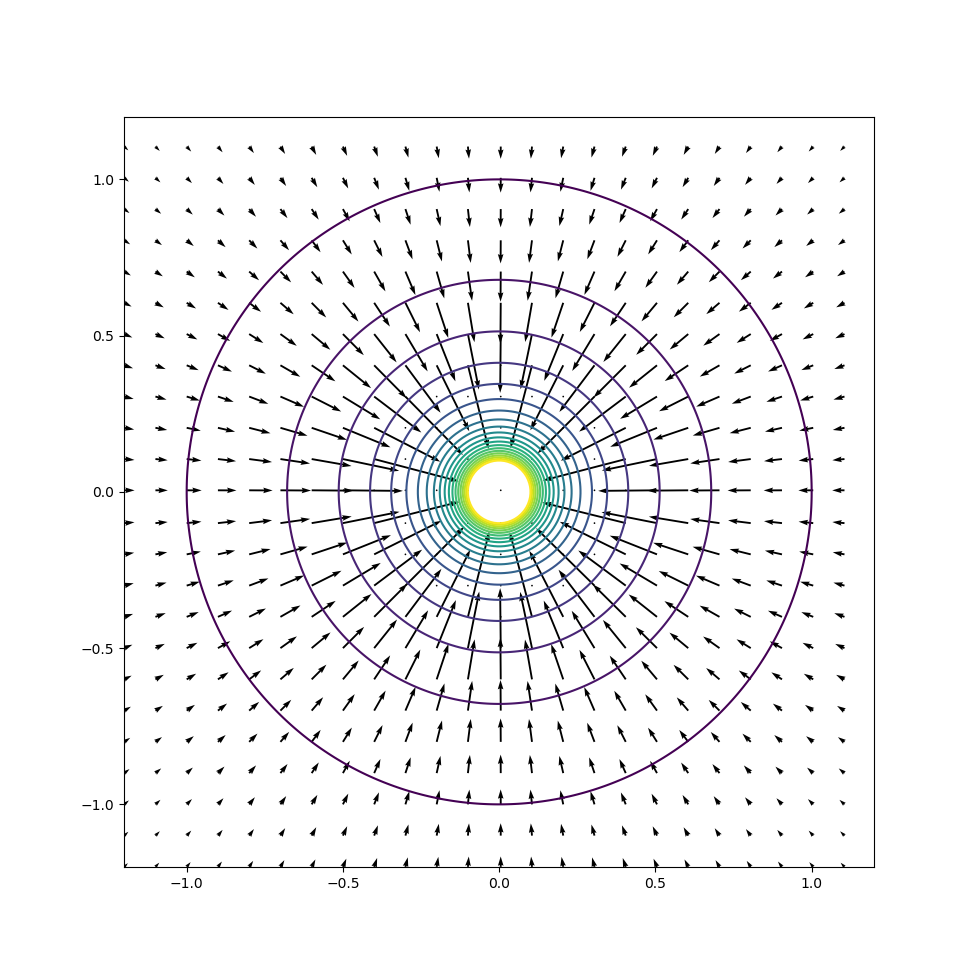
\includegraphics[width=\linewidth]{VP.png} 
		\caption{Gradientenfeld $\nabla V_P$ und Höhenlinien }
	\end{subfigure}
	\begin{subfigure}{0.5\textwidth}
		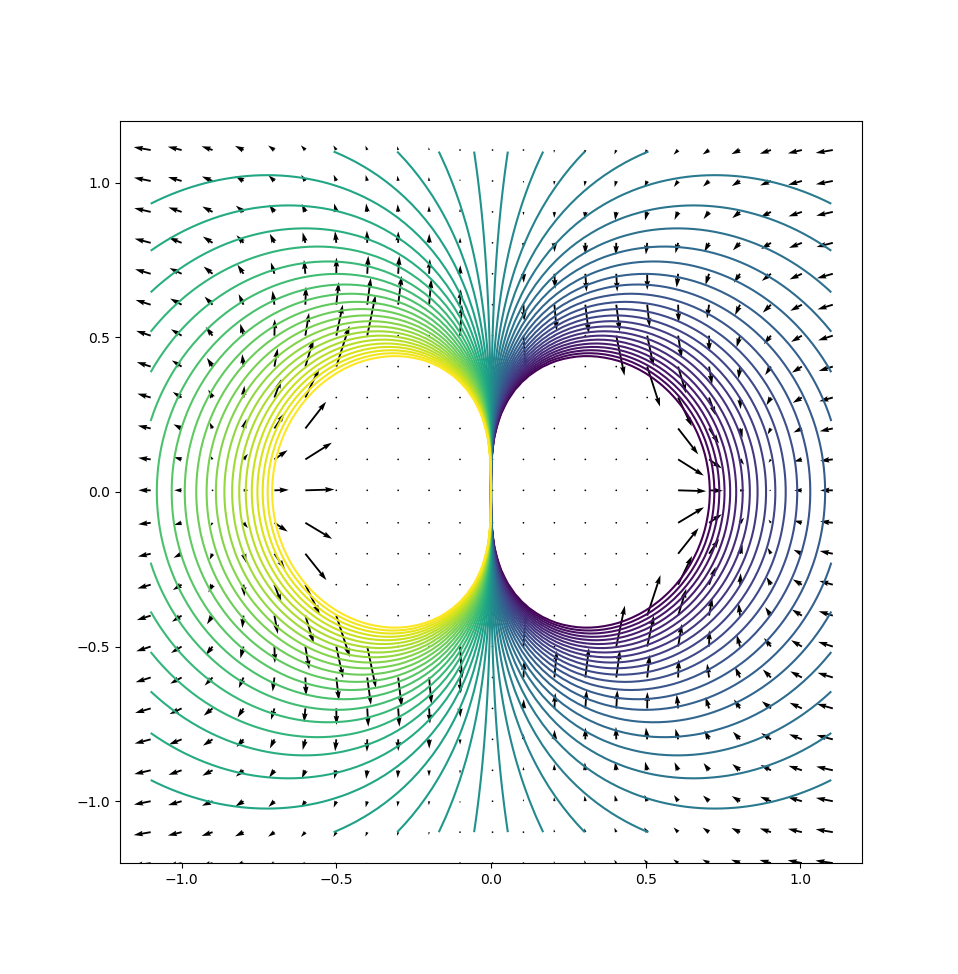
\includegraphics[width=\textwidth]{VD.png} 
		\caption{Gradientenfeld $\nabla V_D$ und Höhenlinien }
	\end{subfigure}
\end{figure}

\end{itemize}


\section{Divergenz}

\begin{itemize}
\item[a)] 
$ \div \vec{F} 
= \div 
	\begin{pmatrix} Kxyz \\ Kxyz \\ Kxyz \end{pmatrix} 
= K( yz + xz + xy ). $ 

\item[b)] 
Wegen $ \vec{\omega} = \begin{pmatrix} 0 \\ 0 \\ \omega \end{pmatrix} $, 
$ \omega \in \R $, ist in Zylinderkoordinaten $ \vec{v} (\vec{r}) = \vec v (r,\ph,z)
= \begin{pmatrix} 0 \\ 0 \\ \omega \end{pmatrix} \times \vec{r} 
= \begin{pmatrix} - \omega \ph \\ \omega r \\ 0 \end{pmatrix} $, also 
$ \div \vec v 
= \frac{1}{r} (- \omega \ph) +0 = - \frac{\omega \ph}{r}. $ 

\item[c)] 
$ \div \vec{v} (x,y,z) 
= \div \sqrt{x^2+y^2+z^2} \vec{a} 
= \frac{x+y+z}{\sqrt{x^2+y^2+z^2}} \vec{a} 
= \frac{x+y+z}{r} \vec{a}. $ 

\item[d)] 
Nach Graßmann: $ \vec a \times (\vec b \times \vec r) = (\vec a \cdot \vec r) \vec b - (\vec a \cdot \vec b) \vec r $. 
Also $ \div \vec{v} 
= \vec a \cdot \vec b - (\vec a \cdot \vec b) \div r = -2 (\vec a \cdot \vec b). $ 

\item[e)]
Es gilt 
\[ \vec E(\vec r) = -Kr^n\hat r = -Kr^{n-1}\vec r = -K (x^2 + y^2 + z^2)^{\frac{n-1}{2}} \vec r. \]
Damit folgt
\[ \frac{d}{dx} E_x = -K\left((x^2 + y^2 + z^2)^\frac{n-1}{2} + 2x^2\tfrac{n-1}{2} (x^2 + y^2 + z^2)^\frac{n-3}{2} \right) = -K(r^{n-1} + (n-1)x^2 r^{n-3})\]
und man erhält analoge Ergebnisse für die Ableitungen von $\vec E$ nach $y$ und $z$. Also
\begin{align*}
 \div \vec E &= -K \left(3r^{n-1} + (n-1)(x^2 + y^2 + z^2) r^{n-3} \right) \\
&= -K \left(3r^{n-1} + (n-1) r^{n-1} \right) \\
&= -(n+2)Kr^{n-1}.
\end{align*}

\end{itemize}



\end{document}